% =====================================================================
% DRAFT -- COMPLETE BUT NOT CLEARED FOR SUBMISSION.
%
% Every section is now written. The stubs that stood here from PROMPT 19 E2
% through PROMPT 21 B are gone, and the \stub{} macro with them: the title, the
% abstract, the structural-prior section, the introduction paragraph and the
% conclusion sentence were all written under PROMPT 21 Part C, after batch C4
% reported.
%
% WHAT STILL BLOCKS SUBMISSION -- both need a human with network access, and
% both are recorded in docs/open-todos.md section 5:
%
%   1. Whether Wiesmayr et al. (arXiv:2210.14103) report the effect of SNR
%      deweighting on the DOWN-WEIGHTED regime. If they do, the 18-of-18 result
%      in Sec. IV-B is anticipated and must be recast as confirmation. The
%      abstract phrases it as a measurement, not a discovery, pending that.
%   2. The pilot-curve train-versus-evaluate ambiguity (Sec. IV-G) was never
%      searched. Its novelty is UNSUPPORTED rather than supported.
%
%   Also: the OFDM reference in the related-work paragraph carries
%   \todo{VERIFY CITATION} and renders in red. Its fields could not be
%   confirmed from this container and it must not enter the bibliography until
%   someone reads the paper.
%
% THE RETIRED CLAIM stays retired. The draft once asserted a fifteenfold
% collapse from +1.209 dB to +0.078 dB. The experiment meant to establish it
% was invalid -- arms trained with init='random' against arms trained with
% init='spectral' (reports/p16/validity.csv, reports/p15/PART_A.md) -- and the
% framing was wrong independently of that: +1.209 is the SMALLEST of its three
% seeds and +0.078 the LARGEST of its three, with a sign that survives neither
% a change of seed nor of pooling rule. The paper now reports a change of
% category across three designs, not a ratio, and "fifteen" appears nowhere.
%
% The framing, and what may and may not be claimed, is in
%     docs/paper2-thesis.md
% Do not restore this file from git history without reading that first.
% =====================================================================
\documentclass[journal]{IEEEtran}
\IEEEoverridecommandlockouts

\usepackage{amsmath,amssymb,amsfonts}
\usepackage{graphicx}
\usepackage{booktabs}
\usepackage{url}
\usepackage{xcolor}

\newcommand{\todo}[1]{\textcolor{red}{\textbf{[TODO: #1]}}}

\DeclareMathOperator{\rank}{rank}
\newcommand{\bG}{\mathbf{G}}
\newcommand{\bS}{\mathbf{S}}
\newcommand{\bB}{\mathbf{B}}
\newcommand{\bW}{\mathbf{W}}
\newcommand{\bZ}{\mathbf{Z}}
\newcommand{\bg}{\mathbf{g}}
\newcommand{\CN}{\mathcal{CN}}
\newcommand{\Hank}{\mathcal{H}}

\begin{document}

% Title written under PROMPT 21 C2, after the results and the abstract body.
% It is constrained by the decision rule committed in reports/p21/PREREG_P31.md
% BEFORE batch C4 ran: the EQUIVALENT branch fired (|m| = 0.121 <= 0.50 and
% m - 2s = -0.141 <= 0), so the log loss does NOT improve on published work and
% the title may claim an attribution finding with a replication attached -- and
% nothing more. "Training Adequacy Confounds" names what the paper establishes;
% it does not claim the loss imbalance, which is wiesmayr2023bler's.
\title{Training Adequacy Confounds the Evaluation of\\
Structural Priors in Unrolled Channel Estimation\\
for Rydberg Atomic Receivers}

\author{Abdullah~Haatim%
\thanks{A.~Haatim is with the Department of Electrical and Electronics
Engineering, Birla Institute of Technology and Science, Pilani~--- Pilani
Campus, India (e-mail:
f20220519@pilani.bits-pilani.ac.in).}}

\maketitle

\begin{abstract}
Adding a structural prior inside an unrolled channel estimator usually improves
the reported metric, and the improvement is usually credited to the prior. We
show that in magnitude-only channel estimation for Rydberg atomic receivers
this evidence is not decisive, because a known training pathology manufactures
it. A per-sample normalized error averaged over a wide SNR range is dominated
by its low-SNR tail; here that amounts to $89.7\%$ of the gradient below
$5$~dB, leaving the high-SNR regime underfitted, so any mechanism that helps
there appears to supply information. We propose a matched-adequacy control:
measure the per-bin gradient share, retrain both the structured and the
unstructured arm with the imbalance removed, and re-measure. Applied to our own
Hankel-structured estimator over three training designs and three seeds each,
the structural advantage at SNR~$\ge5$~dB is $+1.286$~dB under the conventional
loss, $+0.020$~dB when both arms are retrained on the regime of interest, and
$-0.177$~dB when the loss is corrected instead --- positive, absent, and
negative with nothing changed but how training distributed its effort. Two
corrections that share no machinery agree, and a per-bin sign pattern survives
where no scalar does. Correcting the loss is itself a published remedy, and we
measure what it is worth here: $+2.171$~dB at SNR~$\ge5$~dB over three seeds,
improving every one of eighteen bin-by-seed cells including the two the
weighting penalizes most. A log-domain loss needing no bin edges is a simpler
alternative that is no better. Separately, pilot efficiency and pilot-count
generalization are distinct quantities differing by $2.231$~dB. Results are
simulation only.
\end{abstract}

\begin{IEEEkeywords}
Algorithm unrolling, channel estimation, evaluation methodology, phase
retrieval, Rydberg atomic receiver, structural priors.
\end{IEEEkeywords}

\section{Introduction}

\IEEEPARstart{U}{nrolling} an iterative estimator into a trained
network~\cite{gregor2010,monga2021} has become standard for channel estimation,
including for Rydberg atomic receivers, where the magnitude-only readout makes
the problem one of phase retrieval~\cite{xiao2026,cui2025}. A recurring next
step is to add an explicit structural prior --- a low-rank projection, a
sparsity constraint --- inside the unrolled loop, and to report the resulting
improvement as evidence that the prior supplies information the network lacks.

This paper argues that such evidence is usually not decisive, and that the
reason is a convention so widespread it is rarely stated: the training loss is
a per-sample normalized error, averaged over a training set spanning a wide
SNR range.

\textbf{This is a finding about evaluation practice, and we did not arrive at
it as critics.} We built a Hankel-structured unrolled estimator, measured an
advantage at high SNR, and believed it. The control described in
Sec.~\ref{sec:protocol} was run to characterize that advantage, not to remove
it. The first casualty of the protocol we propose was our own method, and we
report it because a result that survives an author's attempt to keep it is
worth more than one that was never tested.

\textbf{Related work on SNR-dependent loss design.} The imbalance itself is
known and we do not claim it. Wiesmayr \emph{et al.}~\cite{wiesmayr2023bler}
state it directly for ML-assisted detection and decoding: a system learns one
parameter set while operating over a range of SNRs, the training data is
sampled from that range, and the aggregate loss is then dominated by the
low-SNR samples, because a small relative improvement at low SNR moves the cost
further than a large one at high SNR. They propose SNR deweighting as the
remedy. Work on deep OFDM channel estimation has separately examined training
on SNR-restricted samples, reporting the expected trade of low-noise accuracy
against high-noise accuracy.\todo{VERIFY CITATION: arXiv:2401.05436, fields
unconfirmed} What we take from that line of work is the mechanism and the
remedy. What is not taken from it, and what this paper is about, is the
consequence for \emph{attribution}: that a known training defect manufactures
apparent evidence for a structural prior, so that crediting the prior without
controlling for the defect is unsound. Wiesmayr \emph{et al.} identify the
pathology and fix it; they do not ask what it does to the evidence.

\textbf{Contributions.}
\begin{enumerate}
\item An attribution decomposition of an unrolled estimator's gain, separating
the learned filter, the attention block, and unrolling itself against a matched
non-unrolled control.
\item The consequence of a known training pathology for \emph{attribution}:
per-sample normalized error over mixed SNR concentrates the gradient at low
SNR~\cite{wiesmayr2023bler}, so any mechanism that improves high-SNR behaviour
will appear to add information, and a structural prior credited on that
evidence is credited for the training's failure rather than its own
contribution. We give a matched-adequacy protocol that separates the two.
\item Two properties of the structural contrast that a scalar hides: a per-bin
sign pattern that replicates across training designs and seeds, and a
dependence of the reported sign on the averaging window.
\item Confirmation that the known remedy~\cite{wiesmayr2023bler} transfers to
unrolled magnitude-only estimation, gaining $+2.171$~dB at SNR~$\ge5$~dB over
three seeds --- with a gain in every bin of every seed, including the two bins
the weighting penalizes most.
\item A demonstration that pilot efficiency and pilot-count generalization are
distinct and are conflated by a single reported curve.
\item A measurement of the same structural prior under three training
designs, three seeds each: its advantage is $+1.286$~dB under the conventional
loss, $+0.020$~dB when both arms are retrained on the regime of interest, and
$-0.177$~dB when the loss is corrected instead.
\end{enumerate}

\textbf{What the control did.} Under the conventional loss the prior is worth
$+1.286$~dB at high SNR, on three seeds, positive under every statistic we
tried. Retraining both arms on the high-SNR range leaves $+0.020$~dB, with one
seed of three significantly negative. Correcting the loss instead --- leaving
the training range untouched --- leaves $-0.177$~dB, negative on every seed.
The quantity does not shrink by a factor; it stops keeping its sign. Two
corrections that share no machinery agree, which is why we read the training
design as the cause rather than an accident of either control.

\section{System Model and Estimator}

An $N$-element uniform linear array serves $K$ users over $P$ pilots. With
$\bG\in\mathbb{C}^{N\times K}$, pilots $\bS$, known reference beam $\bB$ and
noise $\bW$, the receiver observes magnitudes only,
\begin{equation}
\bZ=\left|\bG\bS+\bB+\bW\right|,\qquad \bW_{np}\sim\CN(0,\sigma^2).
\label{eq:fwd}
\end{equation}
Each user's channel is a sum of $L_k$ plane waves on the array manifold,
with $L_k\sim\mathcal{U}\{3,7\}$~\cite{xu2025} and angles drawn uniformly on
$(-90^\circ,90^\circ)$ (Table~\ref{tab:params}); this is a geometric ULA model,
not a clustered one. The
classical baseline is an expectation--maximization Gerchberg--Saxton iteration
(EM-GS)~\cite{gerchberg1972}; the unrolled estimator
(``URformer'') replaces $T$ iterations with $T$ learned layers, each a
data-consistency step followed by a learned filter, a gate, and a
Transformer block across users~\cite{xiao2026}.

We implement this estimator faithfully on the geometric ULA model of
\eqref{eq:fwd} rather than reproducing any published result; the operating
point differs. Nothing here should be read as a reproduction or a validation of
prior work, nor as a critique of any specific paper. The convention we examine
is near-universal, and our own estimator uses it.

\textbf{The reference curve is genie-aided.} Where a reference appears, it is
an unstructured least-squares estimate formed from the \emph{true} phase of
the noiseless field. It is not a bound: it presumes information no receiver
has, and being restricted to unstructured least squares it can be passed by an
estimator that exploits channel structure --- which we in fact observe below
$5$~dB in Sec.~\ref{sec:balanced}.

\section{Attribution and the Matched-Adequacy Protocol}
\label{sec:protocol}

\subsection{Where the gain comes from}

Fig.~\ref{fig:attr} decomposes the unrolled estimator's $3.345$~dB
improvement over EM-GS. The learned per-layer filter, $980$ parameters,
contributes
% src: reports/trackD_stage2_report.md:107-110
$0.147$~dB; the attention block contributes the remaining $3.198$~dB, or
$96\%$. The filter's contribution does not grow with data --- it falls
slightly, $0.193\to0.147$~dB from $20$k to $80$k training samples --- which is
what a never-capacity-limited $980$-parameter component should do.

Unrolling is doing real work independently of attention. Against a matched
control that applies one Transformer block to a converged EM-GS estimate
rather than unrolling, the unrolled estimator gains
% src: reports/trackD_stage3_report.md:98
$0.920$~dB, CI $[+0.888,+0.988]$, winning on $86.5\%$ of trials.

\begin{figure}[!t]
\centering
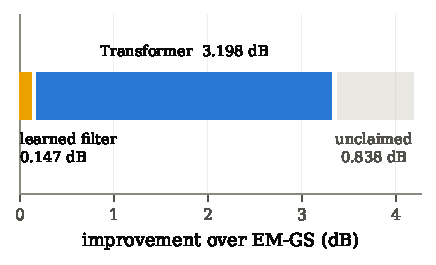
\includegraphics[width=\columnwidth]{fig/fig1_attribution.pdf}
\caption{Attribution of the unrolled estimator's gain over EM-GS at $80$k
training samples. ``Unclaimed'' is the remainder of the genie-aided
least-squares headroom, which is a reference and not a bound.}
\label{fig:attr}
\end{figure}

\subsection{The confound}

The mechanism in this subsection is the one stated
in~\cite{wiesmayr2023bler}; what is new here is its magnitude in an unrolled
magnitude-only estimator, and what it does to attribution.

The training loss is the per-sample normalized error
$\|\hat\bG-\bG\|_F^2/\|\bG\|_F^2$, averaged over a batch drawn across the
whole SNR range. Because the normalized error of a low-SNR realization is
orders of magnitude larger than that of a high-SNR one, this average is
dominated by the low-SNR tail. Measured directly on our estimator,
% src: reports/trackD_stage5_results.json runs.C1_snr_balanced_P20.unweighted_shares
$89.7\%$ of the gradient comes from trials below $5$~dB, and the per-bin
gradient share spans a factor of $30.0$ across the range
(Fig.~\ref{fig:balanced}, upper panel).

The consequence is that the high-SNR regime is systematically underfitted, and
\emph{any} mechanism that improves high-SNR behaviour will appear to add
information. A structural prior is exactly such a mechanism.

\subsection{The protocol}

We propose the following control, which is cheap and which we recommend be run
before any structural prior is credited.

\begin{enumerate}
\item Measure the per-bin gradient share of the training loss. If it is far
from uniform, the regime receiving least gradient is underfitted.
\item Retrain \emph{both} the structured and unstructured arms with training
concentrated on the regime of interest, matching data budget, schedule, seed
and initialization.
\item Re-measure the contrast. What survives is attributable to the prior;
what does not was compensating for training inadequacy.
\end{enumerate}

Applying it, and reporting what it did to our own method: under the
conventional loss the structural advantage over $[5,20]$~dB is
% src: reports/p19/p29_score.json three_seed_mean_ge5_db
$+1.286$~dB, averaged over three training seeds. Retraining both arms on
$[5,20]$~dB alone leaves $+0.020$~dB. Correcting the loss instead, without
narrowing the training range, leaves
% src: reports/p20/p30_score.json three_seed_mean_ge5_db
$-0.177$~dB --- the prior now costs accuracy. Sec.~\ref{sec:prior} gives the
three designs with their seed spreads.

The two corrections share no machinery. One changes which channels the network
sees; the other changes how much each channel contributes to the gradient, on
an unchanged training set. That they agree is what makes the common cause
credible: a single control can always be argued to have broken something
incidental, and two unrelated ones are much harder to explain away.

\textbf{Scope of this negative result.} It holds at $N=32$, $K=3$, this data
budget, and the two pilot counts tested. It is not a general claim that
structural priors cannot help unrolled estimators. Indeed the same prior
applied to the \emph{classical} estimator, where no training adequacy is at
stake, gives a large and stable gain, and under a distribution shift in path
richness the structured network degrades least
% src: reports/trackD_stage5_eval.json C5_path_richness_ood
($+0.48$~dB against $+0.73$~dB). The prior buys robustness here; it is the
in-distribution accuracy claim that does not survive the control.

\section{Numerical Results}
\label{sec:results}

Table~\ref{tab:params} lists the configuration. The reported statistic is the
paired per-trial median within an SNR bin, with bootstrap $95\%$ confidence
intervals over $2000$ paired test realizations.

\begin{table}[!t]
\caption{Configuration.}
\label{tab:params}
\centering
\small
\begin{tabular}{ll}
\toprule
Parameter & Value \\
\midrule
% src: trackD_urformer/config.py:120-129, 273
Array elements $N$ / users $K$ / pilots $P$ & 32 / 3 / 20 \\
Paths per user $L_k$ & $\mathcal{U}\{3,7\}$~\cite{xu2025} \\
SNR (train and test) & $\mathcal{U}[-10,20]$~dB \\
Reference-to-signal ratio & 10~dB \\
Unrolled layers $T$ & 10 \\
Trainable parameters & 1{,}586{,}900 \\
% src: reports/trackD_stage2_report.md
Training samples / epochs & 80{,}000 / 13 \\
Test realizations & 2{,}000 (paired) \\
\bottomrule
\end{tabular}
\end{table}

\subsection{The known remedy transfers to this setting}
\label{sec:balanced}

The confound is a property of the loss, and the remedy for it is already
known~\cite{wiesmayr2023bler}. This subsection reports what it is worth here.
That is a confirmation, not a contribution, and it is placed first only because
the rest of the section is easier to read once the loss is fixed.

We weight each
sample by a static per-bin factor $w(b)=c/m(b)$, where $m(b)$ is the mean
per-sample normalized error in bin $b$ measured once before training, with $c$
set so the weights have unit mean. This requires no schedule, no tuning, and
no change to the architecture.

It works as designed. The realized per-bin gradient share spans a factor of
% src: reports/trackD_stage5_results.json runs.C1_snr_balanced_P20
$1.9$ after balancing against $30.0$ before, and the share below $5$~dB falls
from $0.897$ to $0.427$ against an ideal of $0.5$ --- a slight
over-correction.

The estimation result is better than we predicted, and it is measured on three
seeds rather than one. Against identically-trained unbalanced baselines,
% src: reports/p16/p27_score.json per_seed
balancing gains $+1.902$, $+2.242$ and $+2.369$~dB at SNR~$\ge5$~dB, a mean of
$\mathbf{+2.171}$~dB. Each seed's bootstrap $95\%$ confidence interval
\emph{over test realizations} excludes zero. The spread \emph{over seeds} is a
separate quantity and is reported as one: its standard deviation is
$0.241$~dB, on three seeds and therefore two degrees of freedom, so it is
indicative rather than precise. Taking the conservative combination,
$\text{mean}-2\,\text{SD}=+1.689$~dB, the effect is separated from zero across
seeds.

We had pre-registered a low-SNR \emph{cost} of $-0.10$ to $-0.40$~dB on the
reasoning that the lowest bin's weight falls about eighteenfold. There was no
cost. On the seed for which the prediction was registered the low-SNR change is
% src: reports/trackD_stage5_eval.json P13_balanced_vs_uniform_P20
$+0.135$~dB, CI over test realizations $[+0.101,+0.172]$; across the three
seeds the two lowest bins gain $+0.052$ and $+0.202$~dB on average. Downweighting
the bins that dominated the gradient did not harm them, because they were
over-served rather than merely well-served.

The gap to the genie-aided reference at SNR~$\ge5$~dB falls from $+2.897$ to
$+1.000$~dB. Below $5$~dB the balanced estimator passes that reference by up
to $1.99$~dB, which is consistent rather than anomalous: the reference is
restricted to unstructured least squares, and an estimator that has learned
the channel geometry is not so restricted.

\begin{figure}[!t]
\centering
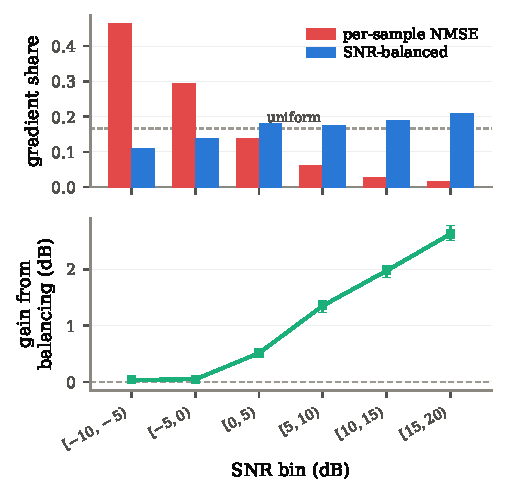
\includegraphics[width=\columnwidth]{fig/fig3_balanced_loss.pdf}
\caption{Cause and effect. Upper: per-bin gradient share under the per-sample
normalized loss and under SNR balancing. Lower: the resulting per-bin gain,
paired per-trial median with bootstrap $95\%$ CI over test realizations, on the
seed for which the prediction was registered.}
\label{fig:balanced}
\end{figure}

\subsection{The correction improves the regime it penalizes}
\label{sec:18of18}

The obvious objection to a reweighting is that it trades one regime for
another: whatever the high-SNR bins gain, the down-weighted low-SNR bins must
have paid. Here they did not, and the check is exhaustive rather than pooled.

Fig.~\ref{fig:allcells} plots every SNR bin for every seed.
% src: reports/p16/p27_score.json bins, per_seed.*.per_bin_db
\textbf{All eighteen bin-by-seed cells favour the balanced loss}, and seventeen
of the eighteen have a bootstrap $95\%$ confidence interval over test
realizations that excludes zero; the single exception is seed~1's $[-5,0)$~dB
bin at $+0.044$~dB, CI $[-0.011,+0.105]$. The three-seed means rise
monotonically across the range, from $+0.052$~dB in $[-10,-5)$ to $+3.120$~dB
in $[15,20)$.

The two lowest bins are the ones that matter for the objection, because the
weighting divides their contribution by about $18$ and $9$ relative to unit
mean. They gain anyway. The correction is therefore not a transfer between
regimes: it improves the quantity it was weighted away from.

We offer a reading of why, as a hypothesis and not as a result. Under the
per-sample loss the gradient was so dominated by the low-SNR tail that the
network was underfitted \emph{everywhere}, spending capacity on realizations
from which little is recoverable. Rebalancing does not move performance from
one regime to another; it stops wasting it. Testing that claim directly would
require an ablation we have not run.

\begin{figure}[!t]
\centering
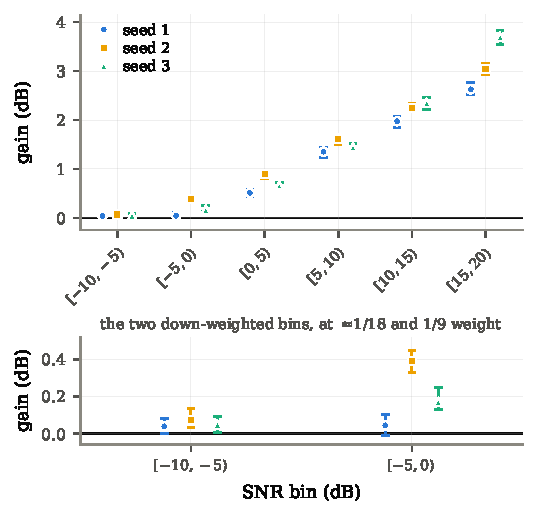
\includegraphics[width=\columnwidth]{fig/fig5_allcells.pdf}
\caption{Every bin, every seed. The gain from SNR balancing, paired per-trial
median with bootstrap $95\%$ CI over test realizations, for each of three
training seeds. All eighteen cells are positive, including the two lowest bins,
whose weights the balancing divides by about $18$ and $9$.}
\label{fig:allcells}
\end{figure}

\subsection{The structural contrast is not a scalar: a per-bin sign pattern}
\label{sec:signpattern}

Reported as one number, the structural gain $\Delta_H$ is a weighted average of
two opposing effects. Per bin, the prior \emph{costs} accuracy at low SNR and
\emph{buys} it at high SNR, and the sign flips exactly once.

\begin{table}[!t]
\caption{Per-bin structural gain $\Delta_H$, three-seed mean, positive = the
prior is better. All eighteen underlying $\Delta_H$ cells of the mixed design
--- three seeds by six bins --- have a bootstrap $95\%$ CI over test
realizations excluding zero. These are a different eighteen from those of
Fig.~\ref{fig:allcells}, which are the gain from balancing the loss.}
\label{tab:signs}
\centering
\small
\begin{tabular}{lrrr}
\toprule
SNR bin (dB) & mixed & SD over seeds & focused \\
\midrule
% src: reports/p19/p29_score.json three_seed_mean_per_bin_db
$[-10,-5)$ & $-0.120$ & $0.036$ & --- \\
$[-5,0)$   & $-0.400$ & $0.103$ & --- \\
$[0,5)$    & $-0.293$ & $0.157$ & --- \\
% src: reports/p17/p28_score.json three_seed_mean_per_bin_db
$[5,10)$   & $+0.457$ & $0.052$ & $-0.173$ \\
$[10,15)$  & $+1.403$ & $0.089$ & $+0.067$ \\
$[15,20)$  & $+2.290$ & $0.082$ & $+0.259$ \\
\bottomrule
\end{tabular}
\end{table}

Two things about Table~\ref{tab:signs} are worth separating.

\textbf{The ordering replicates and the crossing does not.} Every arm we have
measured --- three seeds of mixed-SNR training, three of focused training, and
an earlier arm under the balanced loss --- places every negative bin before
every positive one. On all three mixed seeds the sequence is exactly
$-\,-\,-\,+\,+\,+$ with all eighteen intervals excluding zero. But the bin at
which the sign turns moves by up to two positions between arms. The ordering is
the property that survives; the crossing SNR is not, and neither is any scalar
summary that depends on where it falls.

\textbf{The magnitude collapses under matched adequacy while the ordering does
not.} Comparing the two columns, focused training leaves the shape intact and
reduces the size of every bin by roughly an order of magnitude.

\subsection{The averaging window decides the reported sign}
\label{sec:window}

Because the per-bin contributions have opposite signs, the number one reports
depends on the window the average is taken over --- both which bins are inside
it and how trials are combined within it. Across three seeds of each design:

\begin{itemize}
\item mixed-SNR, restricted to SNR~$\ge5$: $+1.209$, $+1.351$, $+1.298$~dB by
paired per-trial median; $+0.723$, $+0.856$, $+0.901$~dB by ratio of sums.
Positive under both.
\item mixed-SNR, pooled over the whole range: $+0.129$, $+0.225$, $+0.196$~dB
by median; $-0.214$, $-0.146$, $-0.141$~dB by ratio of sums. \emph{Sign
disagreement.}
\item focused training, SNR~$\ge5$: $+0.078$, $+0.057$, $-0.076$~dB by median;
$-0.059$, $-0.077$, $-0.234$~dB by ratio of sums. Negative under ratio of sums
on every seed.
\end{itemize}

\textbf{The reason is measurable and we measured it.} The paired median weights
every trial equally; the ratio of sums weights each trial by its own squared
error. Sorting trials by the no-prior arm's error, the top two deciles carry
$51.2\%$ of the total and contribute $-0.134$~dB, while the remaining eight
contribute essentially nothing. That is not a conditioning effect separate from
SNR: within an SNR bin the rank correlation between the baseline error and
$\Delta_H$ is $-0.009$, $-0.046$ and $+0.147$, against $-0.161$ overall and
$+0.198$ against SNR itself. The sum of squared errors is dominated by low-SNR
realizations, which is exactly where Table~\ref{tab:signs} says the prior costs
accuracy.

\textbf{It is not the mechanism that produces the same symptom in the classical
estimator}, where a selection rule abstains on most trials and pins the median
at zero. The unrolled arm has no such rule: the projection is applied
unconditionally, and it moves the estimate on every one of the $10$ layers of
every one of $2000$ trials on every seed, with no trial anywhere near
inactive.

\subsection{The structural prior under matched adequacy}
\label{sec:prior}

Table~\ref{tab:designs} is the paper's central measurement. The prior, the
architecture, the data budget, the pilot count and the test set are identical
across its three rows. What differs is only how training distributed its
effort.

\begin{table}[!t]
\caption{The structural gain $\Delta_H$ under three training designs, three
seeds each, all arms spectrally initialized. Positive = the prior is better.
Per-seed intervals are over test realizations; the spread is over seeds and is
reported separately. Three seeds give two degrees of freedom.}
\label{tab:designs}
\centering
\footnotesize
\setlength{\tabcolsep}{3.5pt}
\begin{tabular}{lccccc}
\toprule
Training design & $\Delta_H$ & SD$_\text{seed}$ & $\bar{x}-2s$ & sign & RoS \\
\midrule
% src: reports/p19/p29_score.json
Conventional loss & $\mathbf{+1.286}$ & $0.072$ & $+1.142$ & $+\,+\,+$ &
$+\,+\,+$ \\
% src: reports/p17/p28_score.json
Focused $[5,20]$ & $\mathbf{+0.020}$ & $0.083$ & $-0.147$ & $+\,+\,-$ &
$-\,-\,-$ \\
% src: reports/p20/p30_score.json
Balanced loss & $\mathbf{-0.177}$ & $0.150$ & $-0.477$ & $-\,-\,-$ &
$-\,-\,-$ \\
\bottomrule
\end{tabular}
\end{table}

\textbf{Positive, absent, negative.} Under the conventional loss the prior is worth
$+1.286$~dB at SNR~$\ge5$~dB, positive on every seed and under both pooling
rules, and separated from zero by twice the across-seed spread. Retrain both
arms on the high-SNR range alone and it is $+0.020$~dB, with one seed of three
significantly \emph{negative} and the ratio of sums negative on all three.
Correct the loss instead and it is $-0.177$~dB: negative on every seed, under
both pooling rules, with every one of the eighteen per-bin intervals excluding
zero.

We state this as a change of category, not as a factor. A ratio between the
first and last rows would suggest a quantity that shrank; what the table shows
is a quantity that does not keep its sign.

\textbf{Two interventions, one cause.} Focused retraining and loss correction
have nothing in common except that each removes the imbalance of
Sec.~\ref{sec:protocol}. One narrows what the network sees; the other reweights
an unchanged training set. When two unrelated corrections move a measurement
the same way, the common cause is established far more firmly than either could
establish it alone --- and the second is the more pointed of the two, because
it leaves the operating range untouched and so cannot be dismissed as having
simply matched training to the test.

\textbf{What we do not claim.} We have not measured $\Delta_H$ under the
log-domain loss of Sec.~\ref{sec:logloss}: doing so needs a prior-carrying arm
trained under that loss, which we did not train. Three designs are reported,
not four. Nor is this a claim that the Hankel prior is useless in general. It
holds at $N=32$, $K=3$, this data budget and these pilot counts; the same prior
applied to the \emph{classical} estimator, where no training adequacy is at
stake, gives a large and stable gain.

\subsection{A simpler fix that is no better}
\label{sec:logloss}

Per-bin reweighting needs bin edges, a measurement pass before training to
estimate the weights, and a choice of binning. Taking the per-sample error in
decibels before averaging needs none of them: the logarithm divides out the
scale factor exactly, per sample. It is the obvious simplification, so we
tested it on three seeds.

% src: reports/p21/p31_score.json three_seed_mean_log_minus_balanced_db
Against the bin-reweighted arm it gains $+0.121$~dB at SNR~$\ge5$~dB, with an
across-seed SD of $0.131$, so the difference is not separated from zero;
against the conventional arm both fixes gain about the same,
% src: reports/p21/p31_score.json three_seed_mean_log_minus_unbalanced_db
$+2.290$~dB for the log loss. \textbf{The log-domain loss is a simpler
alternative that is no better.} We report it because a reader will ask, and
because a negative answer to an obvious simplification is worth one paragraph.

It is not, however, better balanced. Its realized share of gradient below
$5$~dB is
% src: reports/p21/p31_score.json gradient_shares
$0.317$--$0.329$ against an ideal of $0.5$, where per-bin reweighting reaches
$0.427$; its per-bin span is $3.6$ against the reweighted arm's $1.9$. Dividing
the scale out exactly does not equalize the gradient, because the derivative of
a logarithm is itself inversely proportional to the error.

\textbf{The imbalance is a property of the loss, not of the weights.} The same
log-trained networks, scored under the conventional objective, put
$0.906$--$0.911$ of the gradient below $5$~dB with a span above $40$. A model
trained to be well balanced still exhibits the pathology the moment it is
scored with the objective that causes it --- which is the cleanest statement we
can give that Sec.~\ref{sec:protocol} describes the loss and not the network.

\subsection{Pilot efficiency is not pilot-count generalization}

A pilot-count curve for a trained estimator can mean two different things: one
model trained at some $P_0$ and evaluated at each $P$ (generalization), or a
model trained at each $P$ (efficiency). These are not close.
% src: reports/trackD_stage5_eval.json P14_P10
Trained at $P=10$, the estimator beats the $P=20$ model evaluated there by
$+2.231$~dB pooled, every bin's CI excluding zero. At $P=35$ the corresponding
margin is $+0.635$~dB, so the model generalizes upward in pilot count far
better than downward.

At $5$~dB the matched-trained estimator reaches
% src: reports/trackD_pilot_three_way.json
$-7.52$~dB at $P=10$, within $0.47$~dB of the genie-aided reference, while the
$P=20$ model evaluated there is $2.60$~dB short of it. The clearest single
indication that the curve is tied to its training condition is that the
$P=20$ model is \emph{worse} at $P=25$ ($-11.13$~dB) than at $P=20$
($-11.27$~dB): more measurements, worse estimate. Fig.~\ref{fig:pilots} shows
all three curves together.

This matters for how such curves are reported. The pilot sweep
of~\cite{xiao2026} is described as ``the NMSE performance versus the number of
pilot transmissions $P$, evaluated at a fixed SNR of $5$~dB'', and as
``crucial for assessing the pilot efficiency of each algorithm''; the text does
not state whether the networks were retrained per pilot count. We report that
as a fact about what the paper specifies, and as motivation for stating the
distinction explicitly --- not as a criticism of that work, whose convention is
the ordinary one and which our own earlier curves shared.

\begin{figure}[!t]
\centering
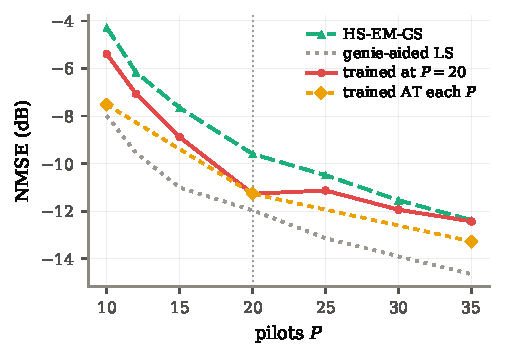
\includegraphics[width=\columnwidth]{fig/fig4_pilots_three_way.pdf}
\caption{Pilot efficiency against pilot-count generalization at $5$~dB, on
identical realizations. The dashed diamonds are separate networks trained at
each $P$; the solid curve is one network trained at $P=20$.}
\label{fig:pilots}
\end{figure}

\section{Conclusion}

A training loss averaged over a wide SNR range is dominated by its low-SNR
tail~\cite{wiesmayr2023bler}; here that amounts to $89.7\%$ of the gradient
below $5$~dB and leaves the high-SNR regime underfitted. The consequence we
draw from it is about evidence rather than about performance: any mechanism
that improves high-SNR behaviour will appear to add information it need not
have supplied, so a structural prior credited on an uncontrolled comparison is
credited for the training's failure. We recommend the matched-adequacy control
be run before a structural prior is credited, and note that it cost us our own
result first.

Two properties of the structural contrast survive that control and a single
number does not report either: the per-bin sign pattern, which replicates
across training designs and seeds while the SNR at which it crosses does not,
and the dependence of the reported sign on the averaging window. Applying the
known remedy~\cite{wiesmayr2023bler} to this setting gains $+2.171$~dB at
SNR~$\ge5$~dB across three seeds and improves every one of eighteen
bin-by-seed cells, including the two the weighting itself penalizes most.

Applied to our own Hankel-structured estimator, the control turns a
$+1.286$~dB advantage into $+0.020$~dB when both arms are retrained on the
regime of interest, and into $-0.177$~dB when the loss is corrected instead ---
three designs, three seeds each, nothing changed but how training distributed
its effort.

\textbf{Limitations.} All results are simulation only, with no measured
hardware and no recorded channel data. They cover the geometric ULA model of
\eqref{eq:fwd} at $N=32$, $K=3$, one data budget and the pilot counts tested;
the negative result about structural priors is scoped to those conditions and
is not a general claim. We establish no fundamental bound: the reference curve
used throughout is genie-aided, presumes phase no receiver observes, and is
passed by our own estimator at low SNR.

\bibliographystyle{IEEEtran}
\bibliography{refs}

\end{document}
